\subsection*{EAN-13 Code}


% normale
Strichcodes sind sich im Allgemeinen sehr ähnlich und unterscheiden sich maximal durch die Strichbreite und -länge. Die Länge ist allerdings für die aktuelle Untersuchung nicht von Interesse, denn diese bietet maximal eine leichte Fehlertoleranz, aber keinen Unterschied in der Erkennungsleistung. Die Strichbreite dagegen ermöglicht eine höhere Robustheit in der Erkennung. Daher untersuchen wir, wie in Abbildung \ref*{fig:eannormal} Bild 1 und 2 zu sehen ist, nur 2 unterschiedliche Strichstärken. 

Strichcodes besitzen keine große Fehlertoleranz, wie z.B. QR-Codes, aber sie besitzen nichtsdestotrotz einen großen Vorteil, nämlich dass eine gute Scanline für die Erkennung ausreicht, wie z.B. in Abbildung \ref*{fig:eannormal} Bild 3.
\begin{figure}[H]
  \centering
  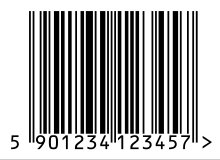
\includegraphics[width=0.30\textwidth]{img/EAN13/perfect_01.jpg}
  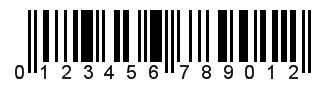
\includegraphics[width=0.35\textwidth]{img/EAN13/perfect_02.jpg}
  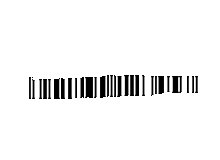
\includegraphics[width=0.30\textwidth]{img/EAN13/compensation_01.jpg}
  \caption{Normale Größe, groß, mit enthaltenem Bild}
  \label{fig:eannormal}
\end{figure}
% \textbf{Bilder einfügen, (klein), normal, groß, (real), (dreckig), mit Bild}

% unscharfe
Bei unscharfen Bildern macht sich die Strichbreite sofort bemerkbar, denn für die normale Breite ist bereits eine leichte Unschärfe (Abbildung \ref*{fig:eanblurry} Bild 1) inakzeptabel. Bei den breiteren Strichen allerdings ist selbst bei einer mehr als 4 mal so hohen Unschärfe noch eine Dekodierung möglich.
\begin{figure}[H]
  \centering
  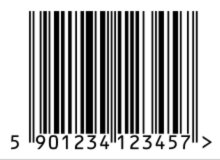
\includegraphics[width=0.30\textwidth]{img/EAN13/blurry_01_07.jpg}
  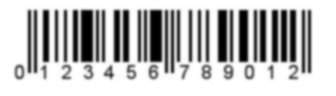
\includegraphics[width=0.35\textwidth]{img/EAN13/blurry_02_3.jpg}
  \caption{Gaußscher Weichzeichner mit 0,7 Pixeln und 3,0 Pixeln Radius}
  \label{fig:eanblurry}
\end{figure}
% \textbf{Bilder einfügen, blurry3, blurry35}

% rotierte
ROTIERT
\textbf{Bilder einfügen, rotate45, rotateface25, rotateface27f, rotateblurry35, rotateblurry40 }

% dunkle
DUNKEL
\textbf{Bilder einfügen, dark98, dark99f, darkface90, darkface95f, blurrydark75, blurrydark80f, blurrydarkrotate90, blurrydarkrotate95f }

% schatten
SCHATTEN

% schräg
SCHRÄG